% 01_introduction.tex

Here is an example of a citation \cite{ref:oetiker1995not}. Citations are included in the \texttt{cited\_works.bib} file.

\blindtext

\subsection{Introduction Section \#1}
\label{sect:intro_1}

For an example of a figure with subfigures, see Fig~\ref{fig:ann_inputs} or~\ref{fig:ann_outputs}.

\blindtext 

\begin{figure}[htbp]
	\begin{subfigure}[t]{.45\textwidth}
		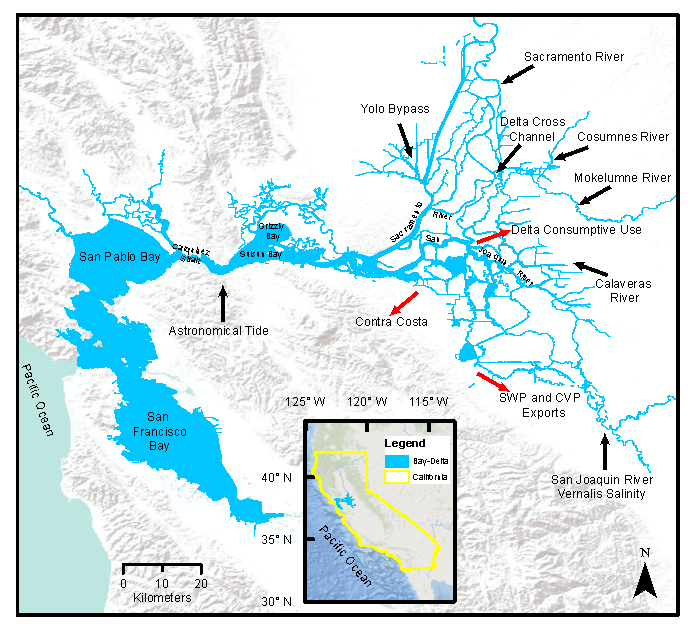
\includegraphics[width=\linewidth]{ann_inputs_he_Aug17.pdf}
		\caption{ANN inputs and input locations.}
		\label{fig:ann_inputs}
	\end{subfigure}
	\begin{subfigure}[t]{.45\textwidth}
		\centering
		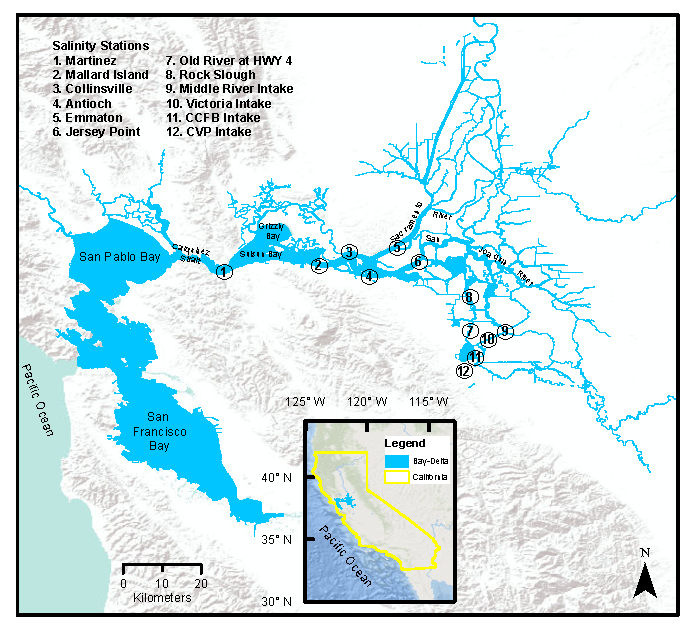
\includegraphics[width=\linewidth]{ann_outputs_he_Aug17.pdf}
		\caption{Locations of the 12 Study Salinity Stations.}
		\label{fig:ann_outputs}
	\end{subfigure}
\caption{ANN input and output locations in San Francisco Bay and Sacramento-San Joaquin Delta Estuary (Bay-Delta Estuary).}
\end{figure}

\subsubsection{Introduction Subsection \#1}
\label{sect:intro_1}
\blindtext
\blindtext

\subsection{Introduction Section \#2}
\label{sect:intro_2}

\blindtext 

\subsection{Introduction Section \#3}
\label{sect:intro_3}
\blindtext
